%
% Problem
\chapter{Problem Formulation} \label{chap::problem}


\section{Omni-wheeled robot} \label{sect::system}
The robot can be represented as a rigid body in a planar space. The location of the robot's \ac{COM} is defined as \lsymb{$\vec p_0\in\R^2$}{Location of the robot's center point} and the yaw of the robot is represeted as \gsymb{$\psi\in\R$}{Roll of the robot}.

Assuming the robot has \lsymb{$n\in\Z_{> 0}$}{Number of wheels} wheels, we can define their 


\section{Dynamic Model}

\newpage
\subsection{Motor Electro-dynamic Identification}

%The motors in our robot are controlled by velocity inputs. We will represent the inputs of the i-th motor as \lsymb{$u_i\in[-1,1]$}{i-th motor input}. The motors are also equipped with encoders from which we can deduce the angle of each wheel, denoted as \gsymb{$\theta_i\in\R$}{i-th wheel angle}.

The motors installed in the robot are IG-42CRGM, which are \SI{24}{\volt} DC motors with a $1/49$ reduction ratio. These motors are controlled by Voltage inputs. DC motors can be characterized by the following equations:
\begin{align}
	V&=K\frac{\dot\varphi}{N} +Ri+L\dott{i}\\
	\tau_{w}&=NKi
\end{align}
Where $V$ and $i$ are the total voltage and intensity through the motor, $N$,$R$,$K$ and $L$ are parameters of the motor, $\tau_w$ is the torque applied to the wheel and $\varphi$ the wheel's angle. If we assume $L$ to be negligible, we get the following expression:
\begin{align}
	\torque_w&=\frac{NKV-K^2\dot\varphi}{R}
\end{align}


%{We can try to identify the model using process model identification. A tool that, given some identification data and a transfer function with unknown parameters, estimates the value of the parameters. We will assume that the relationship between input velocity and the real velocity follow a linear transfer function:
%\begin{equation}
%\frac{\dot{\theta_i}(s)}{u_i(s)}=\frac{K_i}{1+\tau_i s}
%\rightarrow
%\frac{\theta_i(s)}{u_i(s)}=\frac{K_i}{s(1+\tau_i s)}
%\end{equation}
%
%Which corresponds to the following set of ODEs:
%\begin{equation}
%\dot{\theta_i}+\tau\ddot{\theta_i}=u\,K
%\end{equation}
%
%To obtain the identification data we can make the arduino generate a square wave and record the data from the encoder. This will give us data discretized with different time-intervals as the time-interval will depend on the loop size. To get data with equal time-intervals we can set a higher sampling frequency and interpolate the values between each sample.
%
%When identifying the model we saw that the values of $K$ were different for varying amplitudes as we can see in \cref{fig:K_u}.
%
%\todo{Do experiments for higher values of amplitude (when lab is empty)}
%\begin{figure}[h]
%	\centering
%	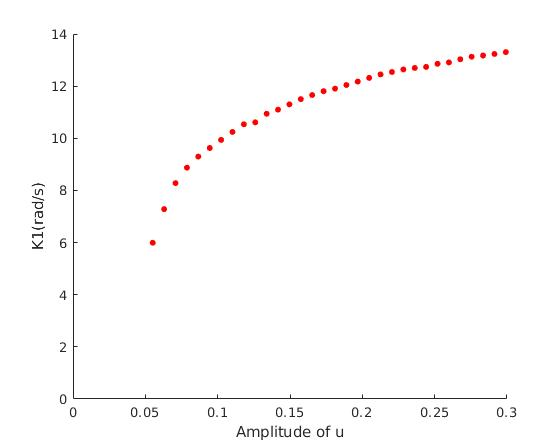
\includegraphics[width=0.31415\textwidth]{Figures/K_u}
%	\caption{Relationship between $K_1$ and the amplitude of $u$}
%	\label{fig:K_u}
%\end{figure}
%
%
%As the relationship looks like it has a vertical and a horizontal asymptote, we will try to model it with a rational function of the form:
%\begin{equation}
%K_i=\frac{a_i\,u_i+b_i}{u_i+c_i}
%\end{equation}
%
%\begin{figure}[h]
%	\centering
%	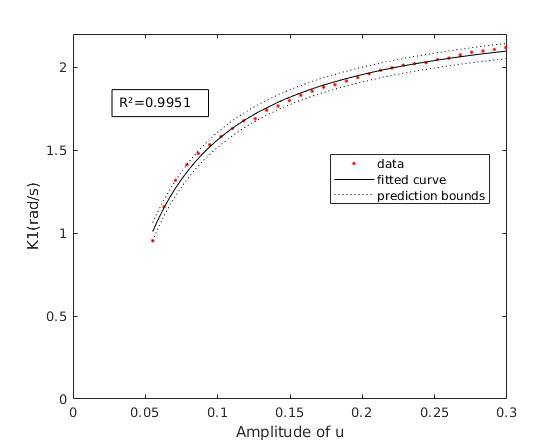
\includegraphics[width=0.31415\textwidth]{Figures/K_u_pred}
%	\caption{Predicted relationship between $K_1$ and the amplitude of $u$}
%	\label{fig:K_u_pred}
%\end{figure}
%\todo{see if $\tau$ depends on u}




